\documentclass[tikz]{standalone}

\usetikzlibrary{intersections}

\begin{document}
	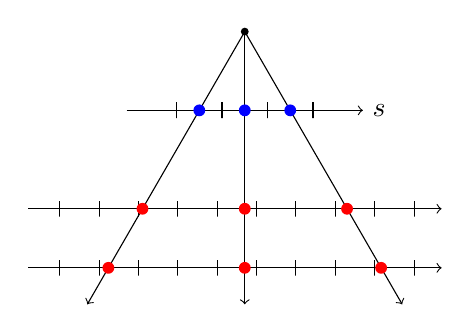
\begin{tikzpicture}[scale = 0.5, baseline, rotate = -90]
	
		% Three rays from camera
		\draw[name path = ray1, ->] (0, 0) -- (30 : 8cm);
		\draw[name path = ray2, ->] (0, 0) -- (0 : {cos(30)*8}cm);
		\draw[name path = ray3, ->] (0, 0) -- (-30 : 8cm);
		
		% Center of projection
		\fill (0, 0) circle[radius = 0.1];
		
		% Image plane
		\draw[name path = imagePlane, ->] (2, -3) -- (2, 3) node[right] {$s$};
		
		% Pixel markers on image plane
		\draw (2, {3 * tan(30) * 2 / 2}) -- ++(0.2, 0) -- ++(-0.4, 0);
		\draw (2, {tan(30) * 2 / 2}) -- ++(0.2, 0) -- ++(-0.4, 0);
		\draw (2, {-tan(30) * 2 / 2}) -- ++(0.2, 0) -- ++(-0.4, 0);
		\draw (2, {-3 * tan(30) * 2 / 2}) -- ++(0.2, 0) -- ++(-0.4, 0);
		
		% Layer axis
		\draw[name path = layer1, <-] (4.5, 5) -- (4.5, -5.5);
		\draw[name path = layer2, <-] (6, 5) -- (6, -5.5);
		
		% Layer set of pixels
		\foreach \x in {1,...,10} 
			\draw (4.5, 10 / 2 * 1 - \x * 1 + 0.3) -- ++(0.2, 0) -- ++(-0.4, 0);
		
		\foreach \x in {1,...,10} 
			\draw (5 + 1, 10 / 2 * 1 - \x * 1 + 0.3) -- ++(0.2, 0) -- ++(-0.4, 0);
		
		% Dots at intersections on image plane
		\fill[name intersections={of=imagePlane and ray1, total=\t}, blue]
			\foreach \s in {1,...,\t}{(intersection-\s) circle[radius = 0.15]};
			
		\fill[name intersections={of=imagePlane and ray2, total=\t}, blue]
			\foreach \s in {1,...,\t}{(intersection-\s) circle[radius = 0.15]};
		
		\fill[name intersections={of=imagePlane and ray3, total=\t}, blue]
			\foreach \s in {1,...,\t}{(intersection-\s) circle[radius = 0.15]};
		
		% Dots at intersections on first layer
		\fill[name intersections={of=layer1 and ray1, total=\t}, red]
			\foreach \s in {1,...,\t}{(intersection-\s) circle[radius = 0.15]};
		
		\fill[name intersections={of=layer1 and ray2, total=\t}, red]
			\foreach \s in {1,...,\t}{(intersection-\s) circle[radius = 0.15]};
		
		\fill[name intersections={of=layer1 and ray3, total=\t}, red]
			\foreach \s in {1,...,\t}{(intersection-\s) circle[radius = 0.15]};
		
		% Dots at intersections on second layer
		\fill[name intersections={of=layer2 and ray1, total=\t}, red]
			\foreach \s in {1,...,\t}{(intersection-\s) circle[radius = 0.15]};
		
		\fill[name intersections={of=layer2 and ray2, total=\t}, red]
			\foreach \s in {1,...,\t}{(intersection-\s) circle[radius = 0.15]};
		
		\fill[name intersections={of=layer2 and ray3, total=\t}, red]
			\foreach \s in {1,...,\t}{(intersection-\s) circle[radius = 0.15]};
		
	\end{tikzpicture}
\end{document}
